\chapter{Oscillateurs, nombres d’occupation et premier champ quantique}

La théorie quantique des champs est le cadre qui décrit pratiquement toute la physique non gravitationnelle connue. Cette affirmation ne signifie pas que tous les problèmes peuvent être résolus. L’atome d’hydrogène est accessible au calcul ; dès que l’on considère un atome comme le bore, le calcul devient déjà bien plus difficile, et celui d’un être humain dépasse de très loin toute capacité réaliste de calcul en théorie des champs. Le cadre peut être fondamental alors même que ses équations restent extrêmement difficiles à résoudre.

Nous allons donc aborder le sujet de la manière la plus élémentaire possible. On l’appelle parfois \emph{seconde quantification}, mais ce nom n’aura guère de sens tant que nous n’aurons pas construit les outils nécessaires. Le chemin le plus court ne part pas d’un champ relativiste, mais de l’oscillateur harmonique. Les ressorts ne sont pas l’essentiel. Ce qui compte, c’est l’algèbre des opérateurs de création et d’annihilation. Dès que l’on répète cette algèbre pour de nombreux modes, un opérateur de création ne signifiera plus simplement ``faire monter un oscillateur d’un niveau'', mais littéralement ``créer une particule.''

\section{L’oscillateur vu comme une algèbre}

Pour un oscillateur, notons \(a^\dagger\) l’opérateur qui augmente l’excitation et \(a\) celui qui la diminue. Les notations \(a_+\) et \(a_-\) sont équivalentes, mais la notation avec dagues anticipe le langage de la théorie des champs. L’état fondamental vérifie
\begin{equation}
a|0\rangle=0,
\end{equation}
et l’opérateur nombre est
\begin{equation}
N=a^\dagger a,
\qquad
N|n\rangle=n|n\rangle.
\end{equation}
Les deux opérateurs d’échelle sont adjoints l’un de l’autre, et leur commutateur essentiel est
\begin{equation}
[a,a^\dagger]=1.
\label{eq:l06-single-commutator}
\end{equation}
Cette petite algèbre constitue presque toute la théorie de l’oscillateur.

On peut retrouver \(a\) et \(a^\dagger\) à partir de combinaisons linéaires appropriées de la position et de l’impulsion. La convention précise dépend des normalisations de \(x\), \(p\), \(m\) et \(\omega\) ; l’énoncé invariant utile ici est que \(a^\dagger a\) reconstitue l’hamiltonien quadratique de l’oscillateur, à une constante additive égale à l’énergie de l’état fondamental près. Ainsi,
\begin{equation}
H=\hbar\omega\left(N+\frac12\right).
\end{equation}
Dans la suite, nous omettons le terme constant et considérons
\begin{equation}
H=\hbar\omega N.
\label{eq:l06-one-oscillator-hamiltonian}
\end{equation}
La fréquence détermine le coût d’une excitation. Augmenter \(n\) d’une unité coûte \(\hbar\omega\) ; diminuer \(n\) d’une unité libère la même quantité d’énergie.

\section{Oscillateurs indépendants en grand nombre}

Considérons maintenant de nombreux oscillateurs, indicés par \(i\). Cet indice n’est qu’un indice, et non l’unité imaginaire. Il peut y avoir un nombre fini ou infini de modes. Un ensemble de ressorts indépendants en donne une image ; les modes normaux d’une corde de violon idéale en donnent une autre. En théorie des champs, c’est le cas d’une infinité de modes qui importe.

L’indépendance a un sens opératoriel. Les opérateurs associés à des sous-systèmes réellement indépendants commutent. Dans le cas contraire, les grandeurs correspondantes ne pourraient pas être mesurées indépendamment et les systèmes ne seraient pas indépendants au départ. Nous avons donc
\begin{align}
[a_i,a_j]&=0, \\
[a_i^\dagger,a_j^\dagger]&=0, \\
[a_i,a_j^\dagger]&=\delta_{ij}.
\label{eq:l06-many-commutators}
\end{align}
Pour \(i\ne j\), tous les opérateurs associés aux deux modes commutent. Pour \(i=j\), la dernière ligne se réduit à l’équation~\eqref{eq:l06-single-commutator}.

Chaque oscillateur possède son propre opérateur nombre et, en général, sa propre fréquence :
\begin{equation}
N_i=a_i^\dagger a_i,
\qquad
H=\sum_i\hbar\omega_i N_i.
\label{eq:l06-many-hamiltonian}
\end{equation}
Un état propre simultané est spécifié par la liste complète
\begin{equation}
|n_1,n_2,n_3,\ldots\rangle,
\qquad n_i=0,1,2,\ldots.
\label{eq:l06-occupation-ket}
\end{equation}
L’entier \(n_i\) est appelé le \emph{nombre d’occupation} du \(i\)e oscillateur. Pour l’instant, ce n’est qu’un terme. Bientôt, il comptera les particules qui occupent un état à une particule, et le nom prendra son sens littéral.

L’état dont tous les nombres d’occupation sont nuls est
\begin{equation}
|0\rangle\equiv|0,0,0,\ldots\rangle,
\qquad a_i|0\rangle=0\quad\text{for every }i.
\label{eq:l06-oscillator-vacuum}
\end{equation}

\begin{classroomqa}\lecturetimestamp{00:15:27}\audiencequestion{Une famille infinie d’oscillateurs correspond-elle au continuum de modes d’un système comme une corde de violon ?}\lecturerresponse{Oui, dans le modèle idéalisé de la corde. Une corde réelle est constituée d’atomes, de sorte que les longueurs d’onde suffisamment courtes finissent par atteindre une coupure microscopique. Le modèle continu motive néanmoins l’ensemble infini de modes utilisé en théorie des champs.}\end{classroomqa}

\section{Pourquoi les coefficients d’échelle sont des racines carrées}

L’action de \(a^\dagger\) doit faire passer un état propre de \(N\) à l’état propre suivant, mais la normalisation laisse place à un coefficient :
\begin{equation}
a^\dagger|n\rangle=c_n|n+1\rangle.
\label{eq:l06-unknown-coefficient}
\end{equation}

\begin{figure}[htbp]\centering
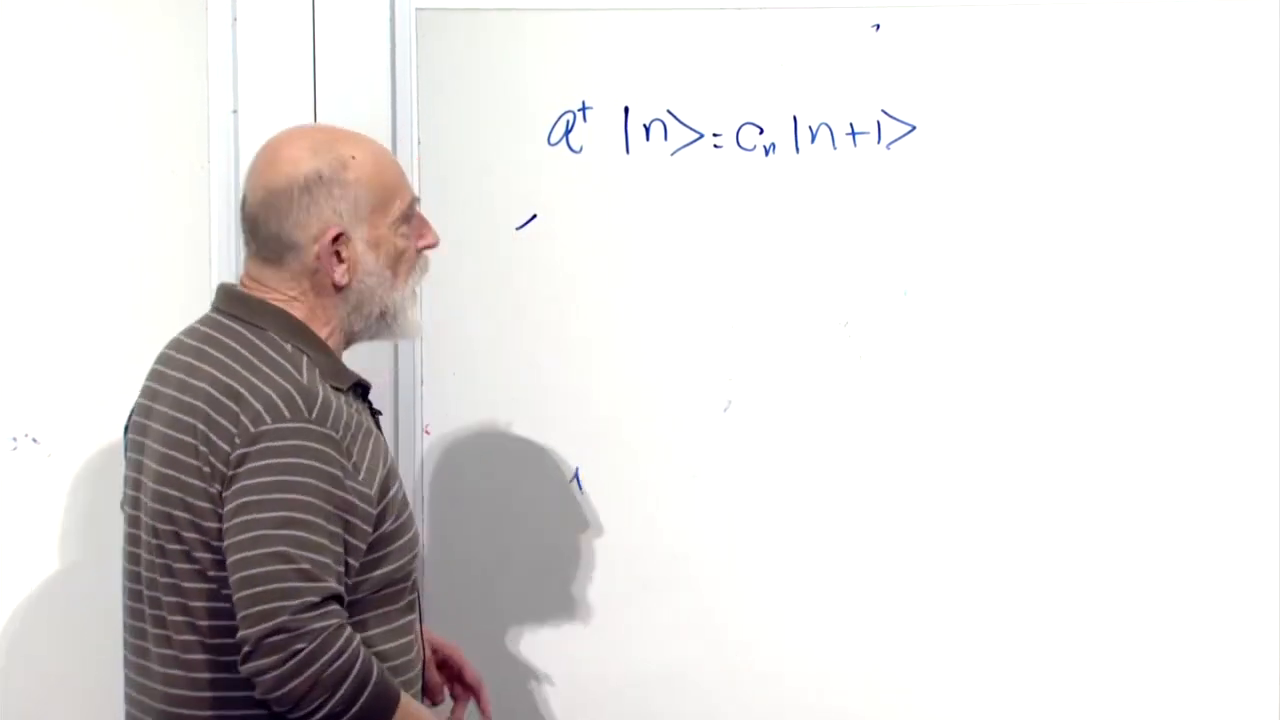
\includegraphics[width=0.9\linewidth]{lecture_06_frame_01.png}\caption{Le coefficient d’échelle est introduit avant que sa normalisation soit établie. L’équation inscrite au tableau est reproduite dans l’équation~\eqref{eq:l06-unknown-coefficient}.}\lectureframe{00:19:38}\end{figure}

Adoptons la convention de phase selon laquelle \(c_n\) est réel. En prenant l’adjoint hermitien, on obtient
\begin{equation}
\langle n|a=c_n\langle n+1|.
\end{equation}
En multipliant les deux relations et en utilisant la normalisation des états de base,
\begin{align}
c_n^2
&=\langle n|aa^\dagger|n\rangle \\
&=\langle n|(a^\dagger a+1)|n\rangle \\
&=\langle n|(N+1)|n\rangle \\
&=n+1.
\end{align}
Par conséquent,
\begin{equation}
a^\dagger|n\rangle=\sqrt{n+1}\,|n+1\rangle.
\label{eq:l06-raising-rule}
\end{equation}

\begin{classroomqa}\lecturetimestamp{00:22:35}\audiencequestion{Pourquoi peut-on poser \(\langle n+1|n+1\rangle=1\) avant de déterminer \(c_n\) ?}\lecturerresponse{Les vecteurs propres sont choisis dès le départ comme une base normalisée. Leur normalisation ne détermine pas celle de \(a^\dagger|n\rangle\) ; l’information qui reste à fixer est précisément le coefficient \(c_n\).}\end{classroomqa}

La règle d’abaissement s’obtient de la même manière :
\begin{equation}
a|n\rangle=\sqrt n\,|n-1\rangle.
\label{eq:l06-lowering-rule}
\end{equation}
Pour \(n=0\), le coefficient s’annule automatiquement ; la règle inclut donc \(a|0\rangle=0\). Avec plusieurs modes, l’opérateur ne modifie que le nombre d’occupation à son propre emplacement :
\begin{align}
a_i^\dagger|n_1,\ldots,n_i,\ldots\rangle
&=\sqrt{n_i+1}\,|n_1,\ldots,n_i+1,\ldots\rangle, \\
a_i|n_1,\ldots,n_i,\ldots\rangle
&=\sqrt{n_i}\,|n_1,\ldots,n_i-1,\ldots\rangle.
\label{eq:l06-multimode-ladders}
\end{align}
Les autres entrées restent inchangées.

\section{Une fonction d’onde n’est pas un champ quantique}

Avant de définir un champ, nous devons le distinguer de la fonction d’onde habituelle. Trois différences organisent cette transition.

Premièrement, une fonction d’onde à une particule
\begin{equation}
\psi(x)=\langle x|\psi\rangle
\end{equation}
est une représentation d’un vecteur d’état. Ce n’est pas une observable en soi. Nous mesurons la position, l’impulsion, le moment cinétique et d’autres opérateurs ; la fonction d’onde fournit les amplitudes à partir desquelles on calcule les probabilités de ces résultats.

Deuxièmement, la fonction d’onde à plusieurs particules dépend des positions de toutes les particules. Pour deux particules dont les vecteurs position sont provisoirement notés \(x\) et \(y\),
\begin{equation}
\psi(x,y)=\langle x,y|\psi\rangle.
\end{equation}
Ici, \(x\) et \(y\) désignent deux particules différentes ; ce ne sont pas les composantes cartésiennes \(x\) et \(y\) d’un même vecteur position. Pour \(N\) particules, l’état est représenté par
\begin{equation}
\psi(x_1,x_2,\ldots,x_N).
\end{equation}

Troisièmement, cette fonction d’onde décrit un nombre fixe de particules. Une fonction d’onde à quinze particules dépend de quinze variables de position et appartient à un espace de Hilbert à quinze particules. À elle seule, elle ne décrit pas un processus où le nombre de particules passe de quinze à quatorze ou à seize.

Un champ quantique inverse ces caractéristiques. C’est un opérateur plutôt qu’un état ; il dépend d’un seul point de l’espace \(x\) et agit sur un espace d’états qui contient tous les secteurs de nombre de particules. L’expression ``un point'' désigne un vecteur position libre de varier. Elle ne signifie pas qu’une valeur numérique unique a été attribuée à \(x\).

Une réserve sera importante par la suite. Le champ \(\Psi(x)\) introduit ci-dessous n’est pas hermitien ; il n’est donc pas lui-même une observable au sens strict. Ses combinaisons hermitiennes sont des observables. L’affirmation provisoire selon laquelle un champ est mesurable est donc précisée, et non abandonnée : les champs sont des fonctions à valeurs opératorielles, et leurs combinaisons hermitiennes représentent des grandeurs mesurables.

\begin{classroomqa}\lecturetimestamp{00:36:52}\audiencequestion{Si le champ est une fonction d’une position, cette position peut-elle varier ? Et qu’est-il advenu de \(y\) dans la fonction d’onde à deux particules ?}\lecturerresponse{Le point \(x\) parcourt tout l’espace. ``Un point'' signifie que l’opérateur dépend d’un seul argument spatial, et non que cet argument est fixé. Dans \(\psi(x,y)\), les symboles \(x\) et \(y\) désignent les positions de deux particules ; on peut aussi les noter \(x_1\) et \(x_2\). Ce ne sont pas deux composantes cartésiennes de l’argument du champ.}\end{classroomqa}

\begin{classroomqa}\lecturetimestamp{00:38:15}\audiencequestion{Quel est le lien entre les descriptions par fonction d’onde à nombre fixe de particules et par champ ? Décrivent-elles des sortes de particules différentes ?}\lecturerresponse{Le lien est la construction centrale que nous allons encore établir. Les particules sont de même nature. Dans ce cours, ce sont des bosons ; les fermions nécessitent une algèbre différente.}\end{classroomqa}

\section{Une particule dans une boîte}

Revenons provisoirement à la mécanique quantique ordinaire à une particule. Plaçons une particule dans une boîte unidimensionnelle. Avec une seule particule, la distinction entre boson et fermion est sans importance : il n’y a pas de seconde particule identique permettant de tester l’échange ou le principe d’exclusion.

Soient
\begin{equation}
\psi_1(x),\ \psi_2(x),\ \psi_3(x),\ldots
\end{equation}
les fonctions propres de l’énergie. Le mode le plus bas est l’onde la plus lisse qui s’annule aux parois. Le mode suivant possède un nœud intérieur, et les modes d’énergie plus élevée oscillent plus rapidement. Pour un puits carré infini idéal de largeur \(L\), une base orthonormée commode est
\begin{equation}
\psi_i(x)=\sqrt{\frac{2}{L}}\sin\!\left(\frac{i\pi x}{L}\right),
\qquad 0<x<L.
\label{eq:l06-box-basis}
\end{equation}
La formule explicite en sinus est une réalisation standard du schéma qualitatif tracé au tableau ; l’argument qui suit ne requiert qu’un ensemble complet d’états à une particule orthonormés.

\begin{figure}[htbp]\centering
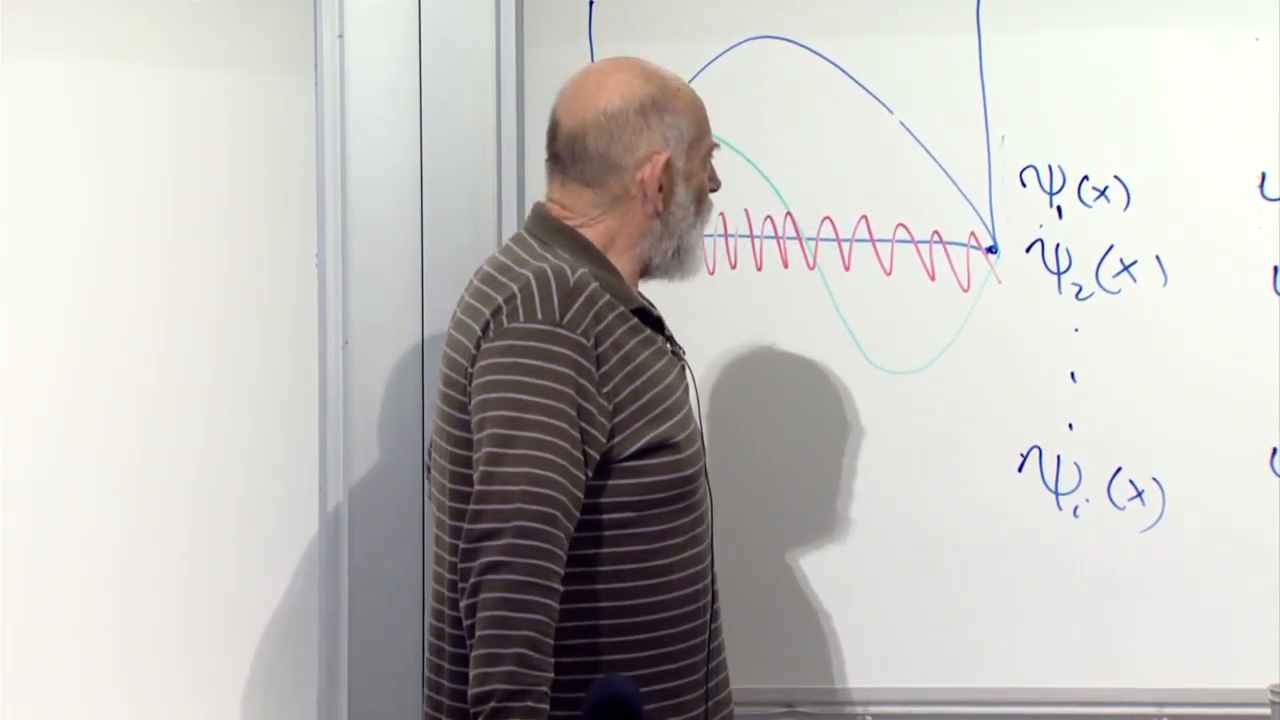
\includegraphics[width=0.9\linewidth]{lecture_06_frame_03.png}\caption{Modes d’une particule dans une boîte, classés par énergie croissante. Le premier mode n’a aucun nœud intérieur, le deuxième en a un, et les modes supérieurs omis oscillent de plus en plus rapidement.}\lectureframe{00:43:10}\end{figure}

La même structure peut être représentée à nouveau sans l’occultation du tableau en direct :
\begin{figure}[htbp]\centering
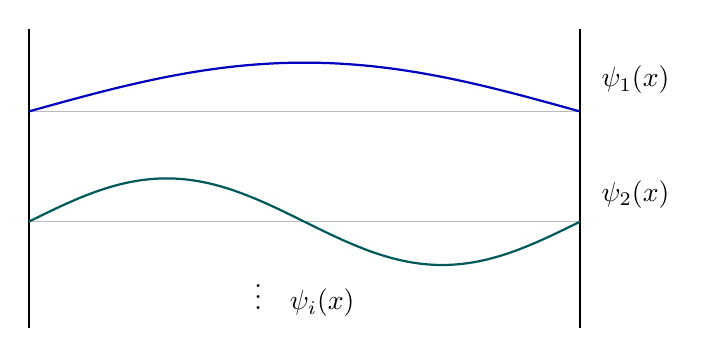
\begin{tikzpicture}[x=1cm,y=1cm]
  \draw[thick] (0,0) -- (0,3.8);
  \draw[thick] (7,0) -- (7,3.8);
  \draw[gray!55] (0,2.75) -- (7,2.75);
  \draw[gray!55] (0,1.35) -- (7,1.35);
  \draw[blue!75!black,thick,domain=0:7,samples=120]
    plot (\x,{2.75+0.62*sin(180*\x/7)});
  \draw[teal!70!black,thick,domain=0:7,samples=120]
    plot (\x,{1.35+0.55*sin(360*\x/7)});
  \node[right] at (7.15,3.15) {$\psi_1(x)$};
  \node[right] at (7.15,1.70) {$\psi_2(x)$};
  \node at (3.5,0.45) {$\vdots\quad \psi_i(x)$};
\end{tikzpicture}\caption{Reconstitution nette du schéma qualitatif des modes dans la boîte. Le décalage vertical sépare les fonctions propres pour en faciliter la lecture ; il ne représente pas une coordonnée physique supplémentaire.}\end{figure}

L’indice \(i\) repère un état à une particule, et non une particule ni le nombre de nœuds. Pour la base de la boîte, \(i\) vaut par coïncidence un de plus que le nombre de nœuds intérieurs. Chaque état possède une énergie \(\varepsilon_i\). En suivant la notation du cours, nous pouvons noter cette énergie \(\hbar\omega_i\), ou simplement \(\omega_i\) après avoir posé \(\hbar=1\).

\begin{classroomqa}\lecturetimestamp{00:39:01}\audiencequestion{L’hypothèse d’indépendance formulée plus tôt était-elle exacte, et l’indice \(i\) pourrait-il désigner les états possibles d’un électron dans un atome ?}\lecturerresponse{Dans la construction à modes indépendants, les relations de commutation entre modes différents sont exactes. L’indice peut désigner des états atomiques à une particule. Toutefois, si les particules interagissent, l’hamiltonien simple à modes indépendants ne suffit plus à décrire le système.}\end{classroomqa}

\begin{classroomqa}\lecturetimestamp{00:40:34}\audiencequestion{La particule dans la boîte est-elle un boson ?}\lecturerresponse{C’est possible, mais avec une seule particule, la statistique n’a pas d’importance. Le principe d’exclusion et l’échange ne prennent sens qu’en présence de plusieurs particules identiques.}\end{classroomqa}

\section{Des modes de la boîte à l’espace de Fock}

Autorisons maintenant un nombre quelconque de bosons identiques dans la boîte. Un certain nombre \(n_1\) peut occuper \(\psi_1\), un certain nombre \(n_2\) peut occuper \(\psi_2\), et ainsi de suite. Un état de base s’écrit donc
\begin{equation}
|n_1,n_2,n_3,\ldots\rangle.
\end{equation}
C’est exactement la notation déjà utilisée pour plusieurs oscillateurs. L’identité est structurelle : associons un oscillateur à chaque état à une particule et identifions le nombre d’excitations de l’oscillateur au nombre de particules qui occupent cet état.

Les bosons sont essentiels ici, car chaque \(n_i\) peut être n’importe quel entier non négatif. Pour les fermions, chaque état à une particule peut être vide ou occupé par une seule particule, jamais par deux ; l’algèbre ordinaire de l’oscillateur ne peut donc pas être reprise telle quelle.

On peut maintenant définir les opérateurs par leur action sur la base des nombres d’occupation. L’opérateur \(a_i^\dagger\) crée une particule dans l’état à une particule \(i\) ; \(a_i\) en enlève une :
\begin{align}
a_i^\dagger|n_1,\ldots,n_i,\ldots\rangle
&=\sqrt{n_i+1}\,|n_1,\ldots,n_i+1,\ldots\rangle, \\
a_i|n_1,\ldots,n_i,\ldots\rangle
&=\sqrt{n_i}\,|n_1,\ldots,n_i-1,\ldots\rangle.
\end{align}
Ce n’est pas une analogie introduite après coup. C’est la définition des opérateurs bosoniques de création et d’annihilation sur cette base. Comme la base engendre l’espace, cette définition détermine leur action sur tout état par linéarité.

\begin{classroomqa}\lecturetimestamp{00:47:11}\audiencequestion{Les \(n_1,n_2,n_3\) sont-ils les états quantiques ?}\lecturerresponse{Les indices \(1,2,3,\ldots\) identifient les états à une particule. Les symboles \(n_1,n_2,n_3,\ldots\) indiquent le nombre de particules qui occupent ces états. Distinguer l’étiquette d’un état de son nombre d’occupation constitue la principale difficulté de notation.}\end{classroomqa}

\subsection{Le rôle de la racine carrée}

Le facteur \(\sqrt{n_i+1}\) ne représente ni une particule supplémentaire ni un processus physique distinct. Il donne à l’opérateur la normalisation et l’algèbre appropriées. Pour un mode,
\begin{align}
a a^\dagger|n\rangle
&=a\bigl(\sqrt{n+1}\,|n+1\rangle\bigr) \\
&=(n+1)|n\rangle,
\end{align}
tandis que
\begin{equation}
a^\dagger a|n\rangle=n|n\rangle.
\end{equation}
Leur différence est donc \(|n\rangle\), comme l’exige \([a,a^\dagger]=1\). En gros, chacun des deux opérateurs d’échelle est d’ordre \(\sqrt n\), puisque leur produit donne l’opérateur nombre, d’ordre \(n\).

\begin{classroomqa}\lecturetimestamp{00:47:52}\audiencequestion{Quelle signification physique concrète faut-il attribuer au facteur racine carrée ?}\lecturerresponse{Il s’agit avant tout d’une normalisation mathématique. Elle garantit que les états d’occupation sont normalisés, que \(a^\dagger a\) a pour valeur propre \(n\) et que les opérateurs d’échelle vérifient le commutateur de l’oscillateur. Parfois, les mathématiques constituent à elles seules le sens dont on a besoin.}\end{classroomqa}

\begin{classroomqa}\lecturetimestamp{00:52:25}\audiencequestion{Les opérateurs de création et d’annihilation ont-ils été définis uniquement par leurs propriétés et leur action sur la base ?}\lecturerresponse{Oui. Les définitions n’ont pas à découler d’une représentation plus fondamentale. Leur intérêt se mesure à leurs conséquences. Définir l’action sur une base complète définit les opérateurs partout, et ces définitions reproduisent les relations de commutation voulues.}\end{classroomqa}

\begin{classroomqa}\lecturetimestamp{00:53:22}\audiencequestion{Pourquoi \(a_i\) fait-il disparaître une particule au lieu de simplement la faire passer à un autre état ?}\lecturerresponse{Parce que \(a_i\) est défini de façon à diminuer le nombre d’occupation de l’état \(i\). La question utile n’est pas de savoir pourquoi une définition est vraie, mais pourquoi elle est utile. Elle l’est parce que l’émission et l’absorption exigent des opérateurs qui modifient le nombre de particules : un photon est créé lors de l’émission de rayonnement et annihilé lors de son absorption.}\end{classroomqa}

L’espace engendré par tous les états à nombres d’occupation est \emph{l’espace de Fock}. Il contient le vide, tous les états à une particule, tous les états à deux particules, et ainsi de suite, sans borne supérieure fixe :
\begin{equation}
\mathcal F=\mathcal H_0\oplus\mathcal H_1\oplus\mathcal H_2\oplus\cdots.
\label{eq:l06-fock-space}
\end{equation}
La notation de somme directe explicite ce que la fonction d’onde ordinaire à \(N\) particules ne montrait pas : tous les secteurs de nombre de particules appartiennent à un seul espace d’états.

\begin{classroomqa}\lecturetimestamp{00:54:56}\audiencequestion{La définition des opérateurs sur les vecteurs propres du nombre d’occupation suffit-elle à les déterminer sur des vecteurs arbitraires, et les commutateurs de l’oscillateur s’ensuivent-ils ?}\lecturerresponse{Exactement. Les vecteurs d’occupation forment une base ; la linéarité étend donc la définition à tout l’espace de Fock. L’action sur cette base vérifie les relations de commutation bosoniques. Chaque état à une particule est représenté par un oscillateur, dont le nombre d’occupation est le nombre de particules dans cet état.}\end{classroomqa}

\subsection{Le vide et l’hamiltonien libre}

Le vide de Fock est l’état où aucun état à une particule n’est occupé :
\begin{equation}
|0\rangle=|0,0,0,\ldots\rangle,
\qquad a_i|0\rangle=0.
\end{equation}
L’expression \emph{état fondamental} peut induire en erreur ici. L’état \emph{à une particule} le plus bas est le mode \(i=1\) ; le vide de Fock ne contient aucune particule, même dans ce mode. Si une particule occupe le mode le plus bas, \(a_1\) peut l’en retirer et ramener le système au vide.

\begin{classroomqa}\lecturetimestamp{00:56:19}\audiencequestion{Qu’est-ce que le vide dans le langage des nombres d’occupation ? L’état à une particule le plus bas est-il occupé ?}\lecturerresponse{Dans le vide, tous les nombres d’occupation sont nuls et chaque \(a_i\) l’annihile. Le mode à une particule le plus bas n’est pas occupé dans le vide. S’il l’était, son opérateur d’annihilation pourrait retirer cette particule.}\end{classroomqa}

Pour des particules sans interaction, l’énergie totale est additive. Si une particule dans l’état \(i\) a une énergie \(\hbar\omega_i\), alors
\begin{align}
H
&=\sum_i \hbar\omega_i N_i \\
&=\sum_i \hbar\omega_i a_i^\dagger a_i.
\label{eq:l06-free-fock-hamiltonian}
\end{align}
On peut l’interpréter de deux façons équivalentes. C’est la somme des énergies des oscillateurs, à raison d’un oscillateur par état à une particule. C’est aussi la somme des énergies à une particule, chacune multipliée par le nombre de particules ayant cette énergie.

Dans la notation de la théorie des champs, \(a_i^\dagger\) est généralement appelé l’opérateur de création et \(a_i\) l’opérateur d’annihilation. Les anciennes notations \(a_+\) et \(a_-\) désignent les mêmes opérateurs.

\section{Éclaircissements avant l’apparition du champ}

Après la pause, plusieurs questions permettent de distinguer le nouveau formalisme de comptage par oscillateurs d’une particule ordinaire se déplaçant dans un potentiel harmonique.

\begin{classroomqa}\lecturetimestamp{01:06:09}\audiencequestion{Les niveaux d’énergie d’une particule dans une boîte ne sont pas équidistants ; où se trouve donc l’oscillateur harmonique ?}\lecturerresponse{Les énergies à une particule \(\omega_i\) n’ont pas besoin d’être équidistantes. Pour chaque mode fixé \(i\), toutefois, les énergies de zéro, une, deux et trois particules sans interaction dans ce mode sont \(0,\omega_i,2\omega_i,3\omega_i\). Cette échelle d’occupation est l’oscillateur. Elle est distincte du cas où une seule particule est placée dans un potentiel d’oscillateur harmonique.}\end{classroomqa}

\begin{classroomqa}\lecturetimestamp{01:08:38}\audiencequestion{Cette construction est-elle liée à la décomposition de Fourier ?}\lecturerresponse{Le lien est profond. Si la base à une particule est formée de modes d’impulsion, les fonctions de mode sont des sinus, des cosinus ou des exponentielles complexes, et les \(a_i\) sont des analogues quantiques des coefficients de Fourier. Une base générale n’a pas besoin d’être trigonométrique, mais le principe du développement est le même.}\end{classroomqa}

\begin{classroomqa}\lecturetimestamp{01:09:07}\audiencequestion{Attribue-t-on la même énergie à toutes les particules, et les interactions sont-elles incluses ?}\lecturerresponse{Les particules qui occupent le même état à une particule ont la même énergie, tandis que celles qui occupent des états différents n’ont généralement pas la même. Pour l’instant, les particules sont libres : elles n’interagissent pas. Les interactions ajouteraient des termes d’énergie potentielle, de sorte que l’hamiltonien ne serait plus seulement la somme additive de l’équation~\eqref{eq:l06-free-fock-hamiltonian}.}\end{classroomqa}

\begin{classroomqa}\lecturetimestamp{01:10:26}\audiencequestion{Qu’est-il advenu du demi-quantum d’énergie du point zéro de chaque oscillateur ?}\lecturerresponse{Il constitue une constante additive dans l’hamiltonien. Une constante commute avec tout opérateur ; elle ne modifie donc pas les équations du mouvement de Heisenberg, et les mesures ordinaires non gravitationnelles dépendent des différences d’énergie. Elle peut compter dans certains cas particuliers, mais elle n’affecte pas la construction développée ici.}\end{classroomqa}

La théorie libre est déjà un outil de comptabilisation d’une puissance remarquable. Elle suit non seulement de nombreuses particules, mais aussi les particules qui changent d’état, apparaissent, disparaissent ou se trouvent dans des superpositions de secteurs de nombre total différent. Les opérateurs ne sont pas de simples symboles de comptage, puisque certaines combinaisons hermitiennes peuvent être mesurées ; le comptage reste néanmoins une première intuition utile.

\begin{classroomqa}\lecturetimestamp{01:14:03}\audiencequestion{Quelles sont les origines historiques de la théorie des champs et de la théorie quantique des champs ?}\lecturerresponse{Un bref parcours historique commence par la représentation physique des champs électrique et magnétique de Faraday, puis par les équations de Maxwell pour les champs classiques. Planck a introduit les quanta d’énergie en étudiant le rayonnement thermique ; Einstein a identifié la quantification au champ électromagnétique lui-même et aux quanta de lumière. Heisenberg, Pauli et surtout Dirac ont ensuite contribué à mettre en place le cadre opératoriel moderne vers la fin des 1920. La catastrophe ultraviolette et la description quantique du rayonnement comptent parmi les problèmes décisifs des débuts. Il s’agit d’un aperçu schématique de l’histoire, et non d’une attribution complète des priorités.}\end{classroomqa}

Ce fil historique explique aussi pourquoi les oscillateurs reviennent sans cesse. Le rayonnement classique dans une cavité se décompose en modes normaux. La quantification de ces modes transforme leurs nombres d’excitation en nombres de photons. Les quanta mathématiques qui occupent les modes deviennent des particules physiques.

\section{L’opérateur de champ bosonique}

Soit \(\{\psi_i(x)\}\) une base complète orthonormée de fonctions d’onde à une particule. Définissons
\begin{equation}
\boxed{\Psi(x)=\sum_i a_i\,\psi_i(x)}
\label{eq:l06-field-annihilation}
\end{equation}
et son adjoint hermitien
\begin{equation}
\boxed{\Psi^\dagger(x)=\sum_i a_i^\dagger\,\psi_i^*(x)}.
\label{eq:l06-field-creation}
\end{equation}

\begin{figure}[htbp]\centering
\includegraphics[width=0.9\linewidth]{lecture_06_frame_04.png}\caption{Développements complets en modes du champ d’annihilation et de son adjoint hermitien. Les équations~\eqref{eq:l06-field-annihilation} et \eqref{eq:l06-field-creation} conservent la même structure opératorielle et de conjugaison complexe sous leur forme composée.}\lectureframe{01:25:15}\end{figure}

Pour toute position fixée \(x\), chaque \(\psi_i(x)\) est un nombre complexe ordinaire. Tout le contenu opératoriel se trouve dans \(a_i\) et \(a_i^\dagger\). Quand \(x\) varie, on obtient un opérateur différent en chaque point de l’espace. C’est en cela que \(\Psi\) est une fonction à valeurs opératorielles.

Si les fonctions de base sont des ondes planes, les équations~\eqref{eq:l06-field-annihilation} et \eqref{eq:l06-field-creation} sont des développements de Fourier quantiques : les coefficients de Fourier classiques sont devenus des opérateurs. Dans une boîte, la base peut plutôt être constituée des fonctions sinus de l’équation~\eqref{eq:l06-box-basis}. Toute base complète orthonormée à une particule convient.

Ni \(\Psi\) ni \(\Psi^\dagger\) n’est hermitien. On peut construire des champs observables à partir de combinaisons hermitiennes, telles que
\begin{equation}
\Psi(x)+\Psi^\dagger(x),
\qquad
i\bigl(\Psi^\dagger(x)-\Psi(x)\bigr),
\end{equation}
et des densités observables seront construites plus tard à partir de produits tels que \(\Psi^\dagger(x)\Psi(x)\). Pour l’instant, il s’agit d’abord de comprendre le rôle des deux champs fondamentaux.

\begin{classroomqa}\lecturetimestamp{01:23:14}\audiencequestion{Comment le membre de gauche peut-il être un opérateur alors que les fonctions de mode à droite sont des fonctions d’onde ordinaires ?}\lecturerresponse{Une fois \(x\) fixé, les fonctions \(\psi_i(x)\) sont des nombres. Les facteurs \(a_i\) sont des opérateurs. Le produit d’un nombre par un opérateur est un opérateur ; la somme en est donc aussi un. Quand \(x\) varie, on obtient toute une famille d’opérateurs.}\end{classroomqa}

\section{Rôle du champ}

Le champ d’annihilation annule immédiatement le vide :
\begin{equation}
\Psi(x)|0\rangle
=\sum_i\psi_i(x)a_i|0\rangle
=0.
\label{eq:l06-field-kills-vacuum}
\end{equation}
Le champ de création nous apprend bien davantage.

Notons \(|i\rangle\) l’état à une particule dont la fonction d’onde est
\begin{equation}
\langle x|i\rangle=\psi_i(x).
\end{equation}
La complétude de la base à une particule donne
\begin{equation}
\sum_i|i\rangle\langle i|=1.
\label{eq:l06-completeness}
\end{equation}
Appliquons cette identité à un état propre de position :
\begin{align}
|x\rangle
&=\sum_i|i\rangle\langle i|x\rangle \\
&=\sum_i\psi_i^*(x)|i\rangle.
\label{eq:l06-position-expansion}
\end{align}
En langage de Fock, un état correspondant à un mode à une particule est
\begin{equation}
|i\rangle=a_i^\dagger|0\rangle.
\end{equation}
En substituant dans l’équation~\eqref{eq:l06-position-expansion},
\begin{align}
|x\rangle
&=\sum_i\psi_i^*(x)a_i^\dagger|0\rangle \\
&=\Psi^\dagger(x)|0\rangle.
\label{eq:l06-local-creation}
\end{align}
Ainsi, \(\Psi^\dagger(x)\) crée une particule localisée en \(x\), tandis que \(\Psi(x)\) en annihile une en ce point. Un état propre de position est localisé sous forme d’une distribution delta et constitue un état généralisé non normalisable ; une particule physique localisée s’obtient en appliquant le champ à un paquet d’ondes normalisable.\editorialnote{Le cours raisonne dans le langage idéal des états propres de position. La précision sur les paquets d’ondes rappelle le sens mathématique usuel sans modifier l’argument.}

\begin{classroomqa}\lecturetimestamp{01:36:26}\audiencequestion{Où se trouve l’information qui précise la nature de la particule créée ? L’état en \(x\) est-il localisé par une distribution delta ?}\lecturerresponse{On associe un champ distinct à chaque espèce de particules ; c’est donc le champ utilisé qui indique l’identité de la particule. L’argument \(x\) précise le lieu de sa création. Dans la base idéale de position, l’état créé est localisé par une distribution delta.}\end{classroomqa}

Parmi les espèces bosoniques figurent les photons, les gravitons, les bosons de Higgs et les gluons, même si les champs réalistes portent aussi des indices internes. Même les photons nécessitent des indices de polarisation. La notation simplifiée du champ scalaire omet ces indices supplémentaires afin de rendre visible le principe de création.

\subsection{Le vide n’est pas le vecteur nul}

L’équation
\begin{equation}
\Psi(x)|0\rangle=0
\end{equation}
contient deux objets très différents désignés par zéro. Le ket \(|0\rangle\) est le vide : un état physique normalisé tel que
\begin{equation}
\langle0|0\rangle=1.
\end{equation}
Le résultat à droite est le vecteur nul. Sa norme est nulle ; il ne peut pas être normalisé et ne représente pas un état physique.

La différence apparaît clairement quand on additionne ces objets. Ajouter le vecteur nul à un état à une particule ne change rien. Ajouter le vide à un état à une particule donne une véritable superposition de secteurs de nombre de particules différents. Avec des coefficients normalisés,
\begin{equation}
|\chi\rangle=\frac{1}{\sqrt2}\bigl(|0\rangle+|1\rangle\bigr)
\end{equation}
autant de chances de trouver zéro particule qu’une seule. Ce n’est pas le même état que \(|1\rangle\).

\begin{classroomqa}
\lecturetimestamp{01:37:23}
\audiencequestion{S’il n’y a aucune particule en \(x\), \(\Psi(x)\) ne fait-il simplement rien ? Que signifie le fait que le résultat soit nul ?}
\lecturerresponse{Il ne renvoie pas l’état initial. Il renvoie le vecteur nul. Le vide est un état normalisé qui décrit l’espace vide ; le vecteur nul est de norme nulle et ne décrit aucun état physique. Tout opérateur agissant sur le vecteur nul renvoie le vecteur nul.}
\end{classroomqa}

\begin{classroomqa}
\lecturetimestamp{01:39:00}
\audiencequestion{Que se passe-t-il si l’on ajoute le vide, plutôt que le vecteur nul, à un état à une particule ?}
\lecturerresponse{On obtient une superposition comportant des amplitudes associées à différents nombres de particules. En revanche, ajouter le vecteur nul laisse l’état à une particule inchangé. Le symbole \(|0\rangle\) désigne une occupation nulle ; il ne signifie pas le vecteur nul.}
\end{classroomqa}

\begin{classroomqa}
\lecturetimestamp{01:41:56}
\audiencequestion{Dans le développement du champ, l’ordre entre une fonction de mode et son opérateur de création ou d’annihilation a-t-il de l’importance ? Les fonctions de mode sont-elles complexes ?}
\lecturerresponse{La fonction de mode est un nombre ordinaire et commute donc avec tout opérateur ; l’ordre n’a donc pas d’importance. En général, les fonctions de mode peuvent être complexes ; le fait qu’une base choisie soit réelle ou complexe dépend du problème de Schr\"odinger à une particule.}
\end{classroomqa}

\subsection{Deux particules et l’émergence de la symétrie bosonique}

Pour créer une particule en \(x\) et une autre en \(y\), appliquons deux fois :
\begin{equation}
|x,y\rangle
=\Psi^\dagger(y)\Psi^\dagger(x)|0\rangle.
\label{eq:l06-two-particle-state}
\end{equation}
Les points peuvent coïncider ou être distincts. Comme les opérateurs de création sous-jacents commutent,
\begin{align}
[\Psi^\dagger(x),\Psi^\dagger(y)]
&=\sum_{i,j}\psi_i^*(x)\psi_j^*(y)
[a_i^\dagger,a_j^\dagger] \\
&=0.
\end{align}
Il s’ensuit que
\begin{equation}
\Psi^\dagger(y)\Psi^\dagger(x)|0\rangle
=\Psi^\dagger(x)\Psi^\dagger(y)|0\rangle.
\label{eq:l06-boson-exchange}
\end{equation}
L’échange de l’ordre des deux particules ne change rien. C’est précisément la symétrie d’échange bosonique. Nous aurions donc pu partir de l’algèbre des oscillateurs et \emph{démontrer} que les particules construites à partir d’opérateurs de création commutants sont des bosons. Les fermions, eux, nécessiteront des opérateurs qui anticommutent.

\begin{classroomqa}
\lecturetimestamp{01:42:37}
\audiencequestion{Comment ajoute-t-on une deuxième particule à l’état à une particule ?}
\lecturerresponse{Appliquez un autre champ de création. Pour l’ajouter en \(y\), agissez avec \(\Psi^\dagger(y)\) à gauche de \(\Psi^\dagger(x)\). On obtient l’état à deux particules de l’équation~\eqref{eq:l06-two-particle-state}.}
\end{classroomqa}

\begin{classroomqa}
\lecturetimestamp{01:46:04}
\audiencequestion{La commutativité des deux champs de création équivaut-elle entièrement à la symétrisation de l’état à deux particules ?}
\lecturerresponse{Oui. Elle rend identique l’état où une particule se trouve en \(x\) et une autre en \(y\) à l’état obtenu après échange des étiquettes. C’est la propriété d’échange qui définit les bosons identiques.}
\end{classroomqa}

\begin{classroomqa}
\lecturetimestamp{01:46:32}
\audiencequestion{Cela signifie-t-il que les particules en \(x\) et en \(y\) doivent être des bosons de même espèce ?}
\lecturerresponse{Oui. Les arguments \(x\) et \(y\) sont des positions, tandis qu’un seul champ décrit une seule espèce. Les espèces différentes, ainsi que les étiquettes supplémentaires comme les deux polarisations du photon, nécessitent des composantes de champ distinctes.}
\end{classroomqa}

\section{Pourquoi la variabilité du nombre de particules est importante}

Si un problème comportait exactement trente-sept particules en permanence, le langage des champs ne serait qu’un moyen facultatif de comptabilisation. Sa véritable force apparaît lorsque des particules peuvent être émises et absorbées, et tout particulièrement lorsque le nombre de particules lui-même est une variable quantique. L’espace de Fock permet des états de la forme
\begin{equation}
|\Phi\rangle
=c_0|0\rangle+c_1|1\rangle+c_2|2\rangle+\cdots,
\qquad
\sum_{n=0}^{\infty}|c_n|^2=1.
\end{equation}
Un champ laser en est un exemple important : ce n’est généralement pas un état doté d’un nombre de photons bien déterminé, mais une superposition de plusieurs secteurs de nombre.

Le lien entre particules et champs est désormais explicite. Les opérateurs de mode comptent les particules dans les états propres de l’énergie et en modifient le nombre ; le champ combine ces opérateurs avec un ensemble complet de fonctions d’onde, de sorte que des particules puissent être créées ou annihilées en des positions spécifiées. L’algèbre des oscillateurs harmoniques est ainsi devenue le langage élémentaire d’un champ quantique bosonique.
